\chapter{System Architecture}
This chapter describes the architecture of the system. An object oriented design
is employed using the key ideas of inheritance and polymorphism. Since there are
different ways to implement polymorphic behaviour and the system was written in
C++ we'll distinguish between the two forms of polymorphism using the same
terminology used in \cite{Stroustrup}. References to \textit{parametric or
compile-time polymorphism} mean the use of templates. References to
\textit{runtime polymorphism} means the use of virtual functions. It should be
noted that there is a slight runtime cost when using virtual functions due to
the extra level of indirection involved. This may be eliminated by the
application of \textit{expression templates} which replace runtime polymorphic
behaviour with compile-time polymorphic behaviour \cite{Veldhuizen95b, LangerKreft}. In the
following chapter references to the \textit{state} of the system can be imagined
as an array the containing the positions and velocities of all the particles in
the system. In general the state of a system can be any differentiable element.
Although references to \textit{pointers} are made in this chapter a shared
pointer system is used in the implementation. 

The system is divided into three separate libraries called Math, Physics and
Render. The Math library contains routines for matrix and vector manipulation
and some core classes that fitted best inside the Math library. The Physics
library contains classes that essentially model a physical phenomenon and return
a force. The Render library consists of a scene graph implementation and an
OpenGL based renderer.

\section{Mass Spring System}
The implementation allowed for an arbitrary configuration of masses and springs.
Initially the Boost Graph Library (BGL) \cite{BGL} was used. Nodes in the graph
stored references to the particles and the edges of the graph stored references
to the springs. After a while the BGL was removed because it was felt to be
overweight for the needs of a mass spring system. For example there was no need
for a shortest path algorithm. Indeed, an interesting question is what physical
meaning can be attributed to the shortest path between 2 particles in the graph,
where the potential energy of the spring gives the edge length.

An algorithm and data structure for computing the forces on all the particles is
given below. It comes from \ref{Eqn:DampedSpring}, which gives the force on a
particle. The data structure allows for a mass spring system of any topology to
be constructed. 

The data structure is a container of tuples. The tuples were created using the
Boost tuple package and contain a particle, followed by a spring and then a
particle. This represents the particle to spring to particle mapping that occurs
in a mass spring system. The data structure, in pseudo-C++ \footnote{It is
pseudo-C++ because namespace qualifiers and extraneous typedefs have been
omitted in order to promote clarity.}, is given in \ref{Lst:PSPTuple}. 

\lstset{language=C++}
\begin{lstlisting}[caption={Particle Spring Particle Tuple},label={Lst:PSPTuple}]
    typedef list < tuple<Particle, Spring, Particle> > 
        PSPContainer
\end{lstlisting}

A type that maps a particle to a force vector is also maintained
\ref{Lst:ParticleForceMap}. This allows for easy look up of the force on a
particle without having to recompute the force, provided that the state of the
system has not changed.

\lstset{language=C++}
\begin{lstlisting}[caption={Particle Force Map},label={Lst:ParticleForceMap}]
    typedef  map<Particle, Force> ParticleForceMap
\end{lstlisting}

An algorithm for computing the forces on each particle using the data structure
above is shown \ref{Lst:MassSpringAlgo}
\lstset{language=Python} 
\begin{lstlisting}[basicstyle={\ttfamily \footnotesize}, caption={Force Calculation for Mass Spring System}, label={Lst:MassSpringAlgo}]
    for (p0, s0, p1) in psp_container:
        relative_direction = p1.position - p0.position
        stretch = norm(relative_direction) - s.rest_len
        relative_velocity = p1.velocity - p0.velocity
        damping = kd*dot(relative_direction, relative_velocity)/
                  norm(relative_direction)
        force = (ks*stretch + damping)*
                (relative_direction/norm(relative_direction))
        pf_map[p0] += force
        pf_map[p1] -= force
\end{lstlisting}	

\section{Solving Differentiable Systems}
At the heart of the dynamics system is a the numerical differential equation
solver. This is the pump that moves the entire state of the system from a point
in time to the next point in time. Since there are many types of numerical 
differential equation solvers it makes sense to define an abstract base class
that incorporates properties common to all differential equation solvers.

\begin{figure}    
    \centering
    \includegraphics[width=0.8\textheight]{DESolver}    
    \caption{\label{Fig:DESolverInheritance}Differential equation solver inheritance diagram}
\end{figure}

The diagram \ref{Fig:DESolverInheritance} shows the \identifier{ODE} class that serves as the
abstract base class for any numerical differential equation solver. The function
\identifier{StepState} implements the algorithm of the specific solver and is
runtime polymorphic. 

The class \identifier{DEStateSource} (see figure \ref{Fig:DEStateSourceDia}) is
an abstract base class that represents any differentiable system. These systems have a
notion of state. In practice this means that they probably have a list of
positions and velocities of the particles in the system. 
The member functions \identifier{SetState},
\identifier{GetState} and \identifier{GetStateDerivative} are runtime polymorphic and are primarily called
by a \identifier{ODE} implementation in its \identifier{StepState} member
function. The function \identifier{GetStateDerivative} tends to be the most
interesting function since it is the one responsible for accumulating the
forces on the particles and solving the equation $\mathbf{F} = m\mathbf{a}$ for
$\mathbf{a}$. For example the class \identifier{CircularConstraint} is able to
maintain the position of a particle a fixed distance from another particle. To
do this it implements the technique described in \ref{SubSec:Pendulum}. The
member function \identifier{GetStateDerivative} accumulates all external forces on the
all particles and calculates the constraint force to work out the state
derivative.  

\begin{figure}
    \centering
    \includegraphics[height=0.3\textheight]{DEStateSourceDia}    
    \caption{\label{Fig:DEStateSourceDia}DEStateSource inheritance}
\end{figure}
 
\section{General Constraints Implementation}
The goal is to implement a set of classes and member functions capable of
solving equation \ref{Eqn:LambdaStable}. This required the definition of an
abstract base class \identifier{Constraint} to serve as a base class for the
various types of constraints (\ref{SubSec:FixedAngleConstraint},
\ref{SubSec:FixedPlaneConstraint}, \ref{SubSec:FixedPostionConstraint},
\ref{SubSec:FDConst}). A class \identifier{ConstraintSystem} was defined to
manage the constraints present in the system and generate the constraint force
vector. 

\subsection{Constraint Classes}
\label{SubSec:ConstraintClasses}
The classes \identifier{FixedDist}, \identifier{FixedAngle},
\identifier{FixedPosition} and \identifier{FixedPlane}, \identifier{FixedVector}
inherit from \identifier{Constraint} as shown in the diagram
\ref{Fig:ConstraintDia}. Each of the these classes provide suitable definitions
for calculating the Jacobian, time derivative of the Jacobian, the legal
velocity, legal position and row size of the Jacobian. The current
implementation requires each instantiation of a \identifier{Constraint} derived
class know the total number of particles in the system as well as row and column
indices that indicate where in the final Jacobian matrix this sub-matrix
should be placed. This is not ideal. The class \identifier{ConstraintSystem}
(see \ref{SubSec:ConstraintSystem}) should manage the positioning of the
individual constraints Jacobians. The member functions shown in the diagram
\ref{Fig:ConstraintDia} are all runtime polymorphic. The number of rows of the
matrices \identifier{Constraint::Jacobian} and
\identifier{Constraint::DJacobian} depends on the type of the constraint. For a
fixed distance constraint the row size of the matrices is 1 since it is a scalar
constraint, whereas a fixed position constraint is a vector constraint and hence
has a row size of 3. The number of columns depends on the number of particles in
the system. Each \identifier{Constraint} derived class needs to be able to
calculate the matrices, the legal position and legal velocity vectors. These
requirements are satisfied by pointers to the particles influenced by the
constraint.

\begin{figure}    
    \centering
    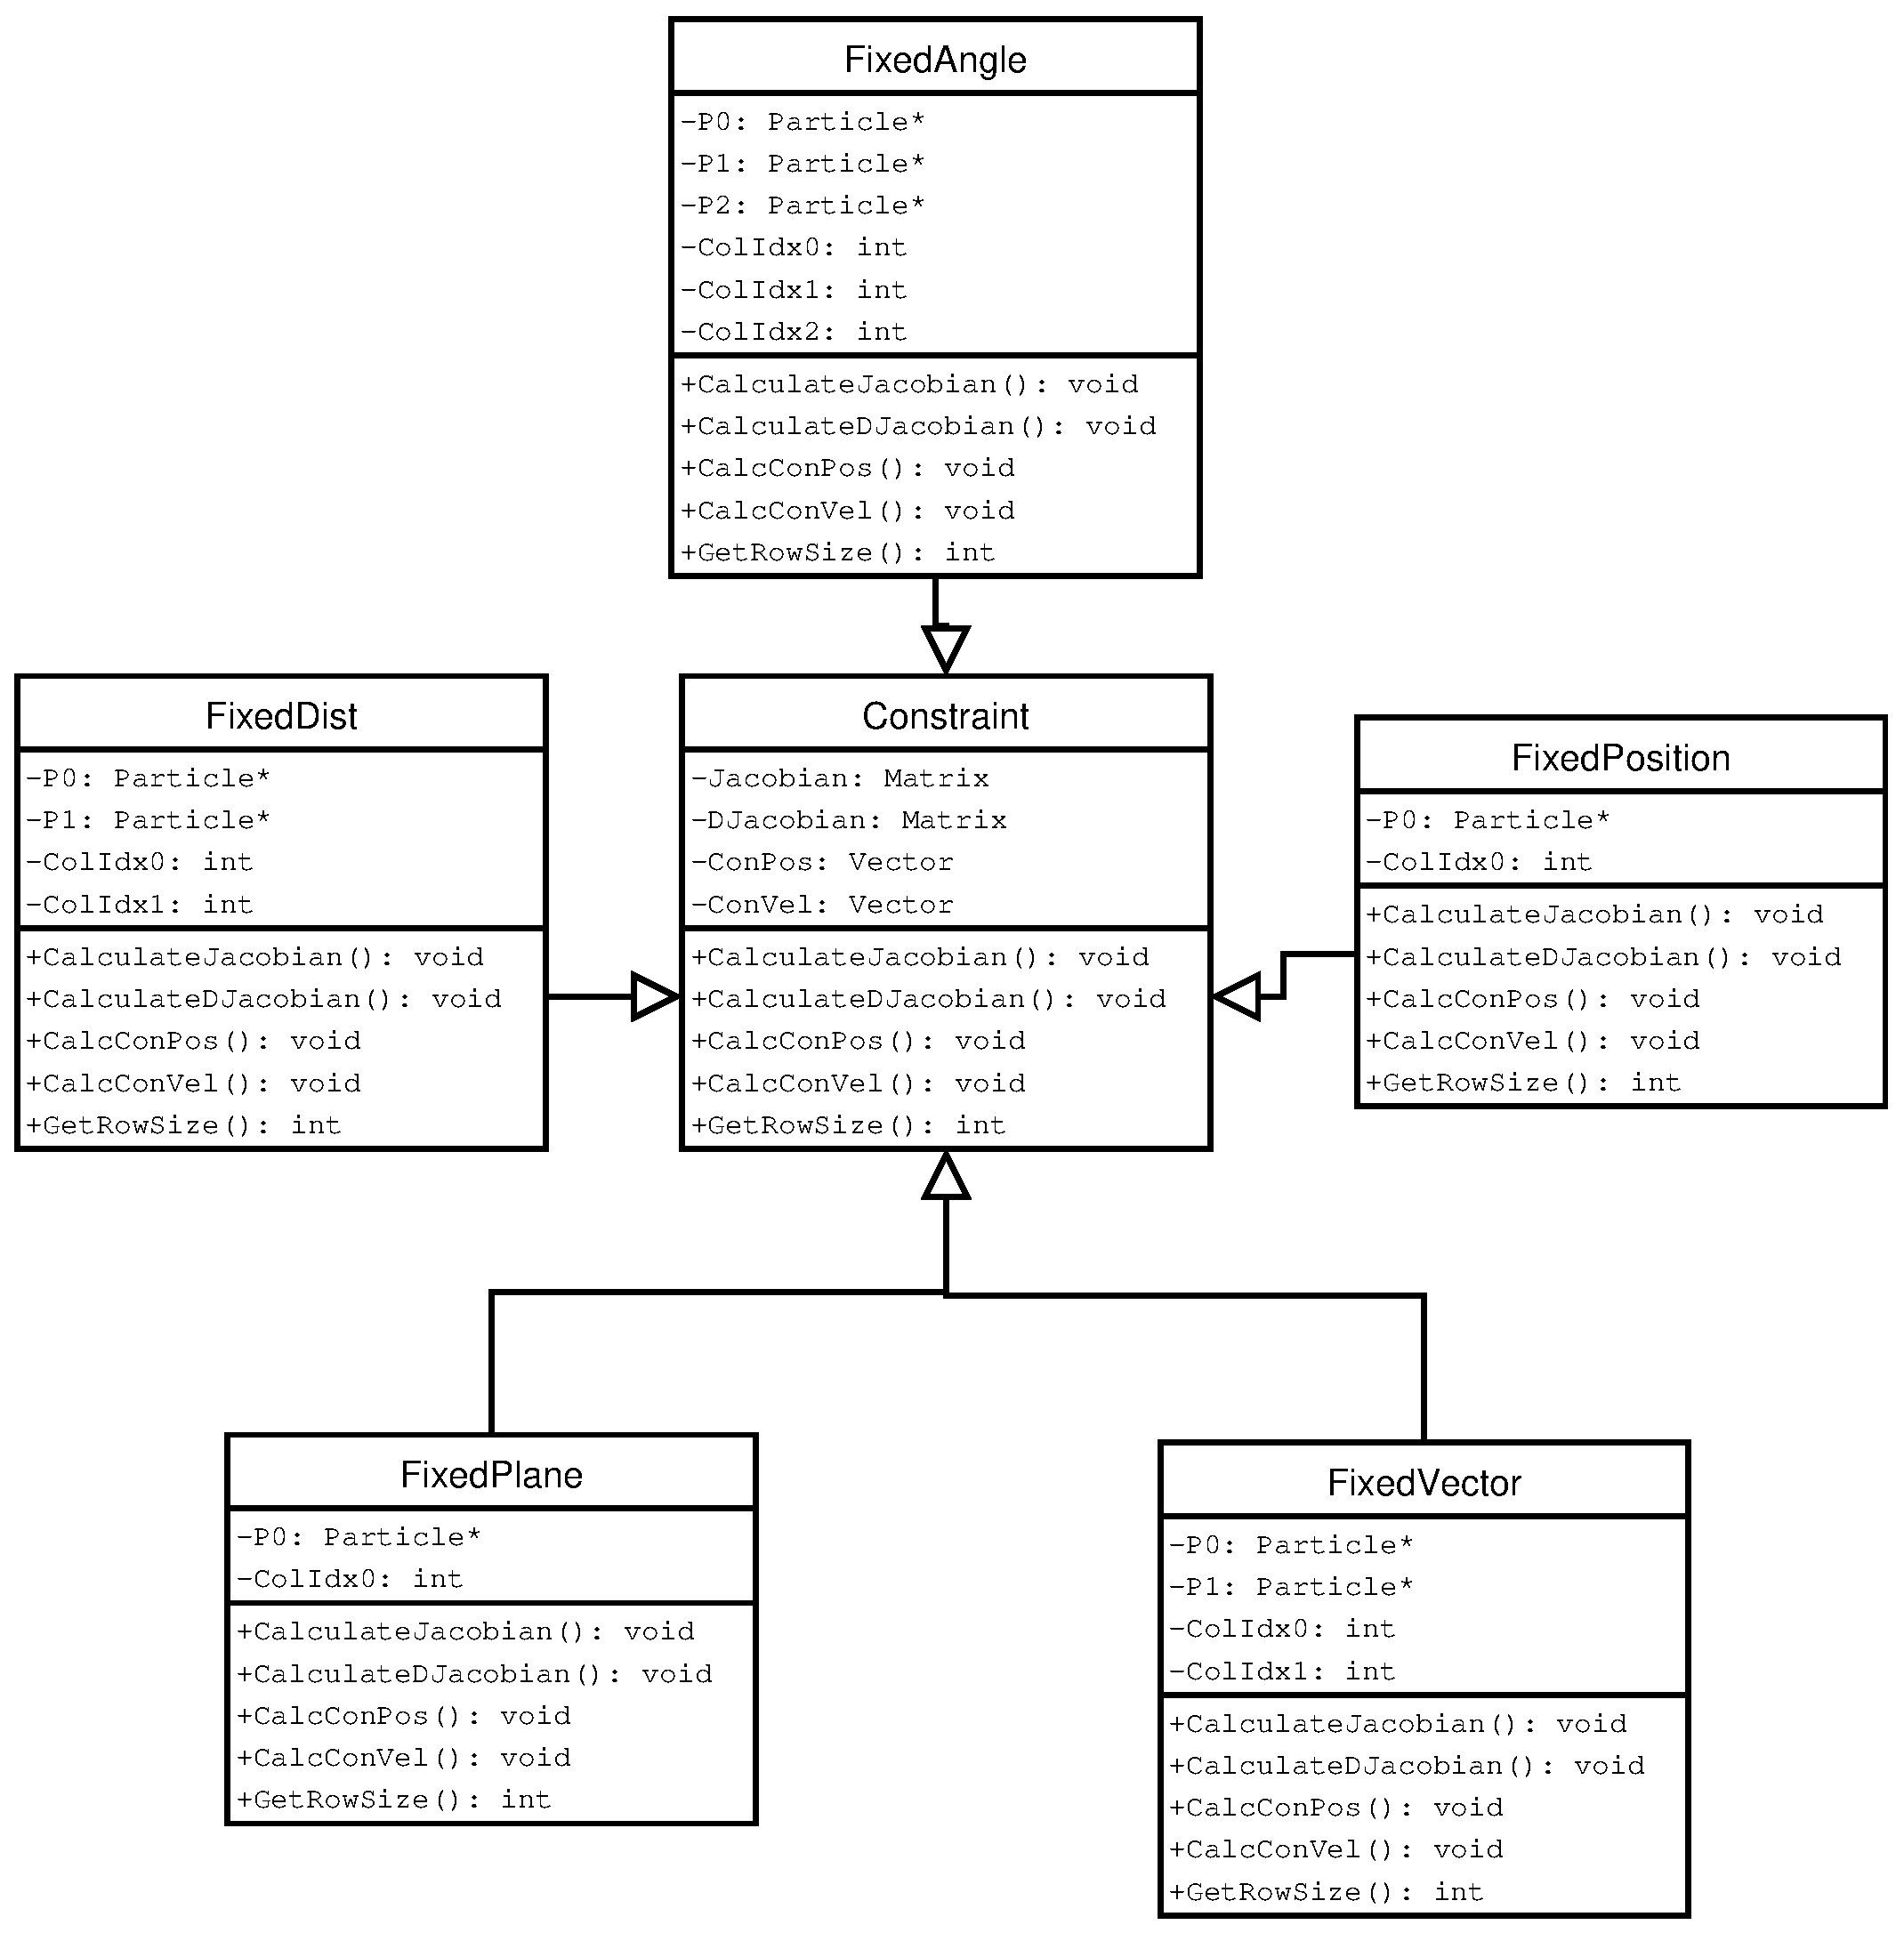
\includegraphics[height=0.8\textheight]{ConstraintDia}    
    \caption{\label{Fig:ConstraintDia}Constraint inheritance}
\end{figure}

\subsection{The ConstraintSystem Class}
\label{SubSec:ConstraintSystem}
The \identifier{ConstraintSystem} manages an array of constraints. It calculates
a global Jacobian matrix (the $\mathbf{J}$ in equation \ref{Eqn:LambdaStable}), by
iterating over all the constraints and calling
\identifier{Constraint::CalculateJacobian}. Similarly it calculates the
derivative of the Jacobian $\dot{\mathbf{J}}$, the constraint $\mathbf{C}$ and
the constraint derivative $\dot{\mathbf{C}}$. Once done it solves equation \ref{Eqn:LambdaStable}
for $\mathbf{\lambda}$ using a biconjugate gradient solver \cite{NumRecipes}
and subsequently the constraint force using equation \ref{Eqn:ConForce}

\begin{figure}
    \centering
    \includegraphics[height=0.2\textheight]{ConstraintSystemDia}    
    \caption{\label{Fig:ConstraintSystemDia}ConstraintSystem Class}
\end{figure}

\section{The Scene Graph}
\label{Sec:SceneGraph}
\subsection{Overview}
A scene graph is a data structure commonly used in software that has to render
and manage data. At its most fundamental level a scene graph groups objects
hierarchically according to their spatial location \cite{Eberly}. The scene
graph implemented uses a tree based representation as shown in figure
\ref{Fig:SceneGraphTree}. In this form each node of the graph, except the root
node, must have only one parent. It is possible to use a directed acyclic graph
where multiple parents are permitted however this is more complex to maintain.
Having multiple parents permits instancing (see figure
\ref{Fig:SceneGraphMultipleParents}) of objects, allowing data to be
shared and thus reducing the memory requirements
\cite{DesigningAPCGameEngine}. Grouping spatially is beneficial because many
objects, like a humanoid character, have a natural hierarchy. Other forms of
grouping are permissible. For example the scene graph implementation used for
this thesis permits grouping based on the material used by the object.  This
permits the renderer to load the materials once for every object that uses that
material. Loading a material can be costly in terms of time. Consider a scene
with many rocks that use the same set of materials.  It is more efficient to
load the material once and then render all the rocks than to load the material
every time a rock needs to be rendered. This is implemented by allowing
materials to also be a node in the graph as shown in figure
\ref{Fig:MaterialNode}.

\begin{figure}
    \centering
    \includegraphics[height=0.3\textheight]{SceneGraphTree}
    \caption{\label{Fig:SceneGraphTree}Scene Graph represented using a tree.}
\end{figure}

\begin{figure}
    \centering
    \includegraphics[height=0.3\textheight]{MaterialNode}
    \caption{\label{Fig:MaterialNode}Material shared by child meshes.}
\end{figure}

\begin{figure}
    \centering
    \includegraphics[height=0.4\textheight]{SceneGraphMultipleParents}
    \caption{\label{Fig:SceneGraphMultipleParents}Scene graph allowing multiple parents.
    This allows instancing where, in this case, the mesh is duplicated at three
    different locations.}
\end{figure}

Operations are performed on the scene graph by traversing the graph. Rendering
is considered to be an operation and the code that does the rendering is wrapped
up in a class of its own. The renderer \footnote{In the code for this thesis
the renderer was implemented using OpenGL.} traverses the
graph in order to draw the objects in the scene. Separating the rendering code
from the scene graph nodes ensures that code that is specific to rendering is
localized to one or two files or in a library of its own. A properly constructed scene graph
allows sharing of data between nodes in order to present data efficiently to the
renderer. 

\subsection{Using the Visitor Pattern}
By doing a depth first traverse of the graph various operations can be
performed on the nodes of the graph. The operations depend on the type of the
object traversing the graph and the type of the node. A base class
\identifier{Node} was defined from which several other classes are inherited
(see figure \ref{Fig:Node} \footnote{Not all the classes that inherit from
\identifier{Node} are shown in the diagram.}). Nodes can be added to a parent
node via the member function \identifier{Node::AddChild}. A base class
\identifier{NodeVisitor} was defined. From it are derived classes that react to
various nodes in different ways when they are encountered during the scene graph
traversal (see \ref{Fig:NodeVisitor}). This can lead to code that uses an
abundance of dynamic casts, for example see \ref{Lst:DynCast}.


\lstset{language=C++}
\begin{lstlisting}[basicstyle={\ttfamily \footnotesize},caption={Dynamic casting example},label={Lst:DynCast}]
void TextureMap::ApplyVisitor(Edge::NodeVisitor* pVisitor)
{
  PreRenderVisitor* pOGLTexGen = dynamic_cast<PreRenderVisitor*>(pVisitor);
  RenderVisitor* pRV = dynamic_cast<RenderVisitor*>(pVisitor);
  ChangeApplyMode* pCAM = dynamic_cast<ChangeApplyMode*>(pVisitor);	
  if (pOGLTexGen)
  {	
    pOGLTexGen->GenerateTexture(this);
  }
  else if (pRV)
  {
    pRV->SetTextureMap(this);
  }
  else if (pCAM)
  {
    pCAM->SetApplyMode(this);
  }
}
\end{lstlisting}

This strategy is undesirable for several reasons. One obvious one is that it
can introduce bugs if you test a base class before a derived class. We use a
simplified implementation of the Visitor pattern described in
\cite{Alexandrescu} to mitigate this problem. This allows us to replace the type
switching at runtime with a type switch that is done at compile time using
overloaded member functions. The class \identifier{NodeVisitor} is augmented
with several overloaded variants of the member functions called
\identifier{Visit} and \identifier{Leave}. All of these functions are pure
virtual which means that any class that inherits from \identifier{NodeVisitor}
(e.g. \identifier{RenderVisitor}) will have to provide an implementation of the
function. The number of variants on \identifier{Visit} and \identifier{Leave} is
dependent upon the number of types of Nodes (i.e. Translate, Material etc..)
that a \identifier{NodeVisitor} derived class can potentially react with. In
some cases a \identifier{NodeVisitor} derived class such as
\identifier{PreRenderVisitor} need not react with every \identifier{Node} type,
however, because it inherits from \identifier{NodeVisitor} and the member
functions \identifier{NodeVisitor::Visit} and \identifier{NodeVisitor::Leave}
are pure virtual the implementation for Node derived classes for which there is
nothing to do is simply a stub function. The diagram in figure
\ref{Fig:NodeVisitorOverloaded} should help clarify the explanation.

\begin{figure}
    \centering
    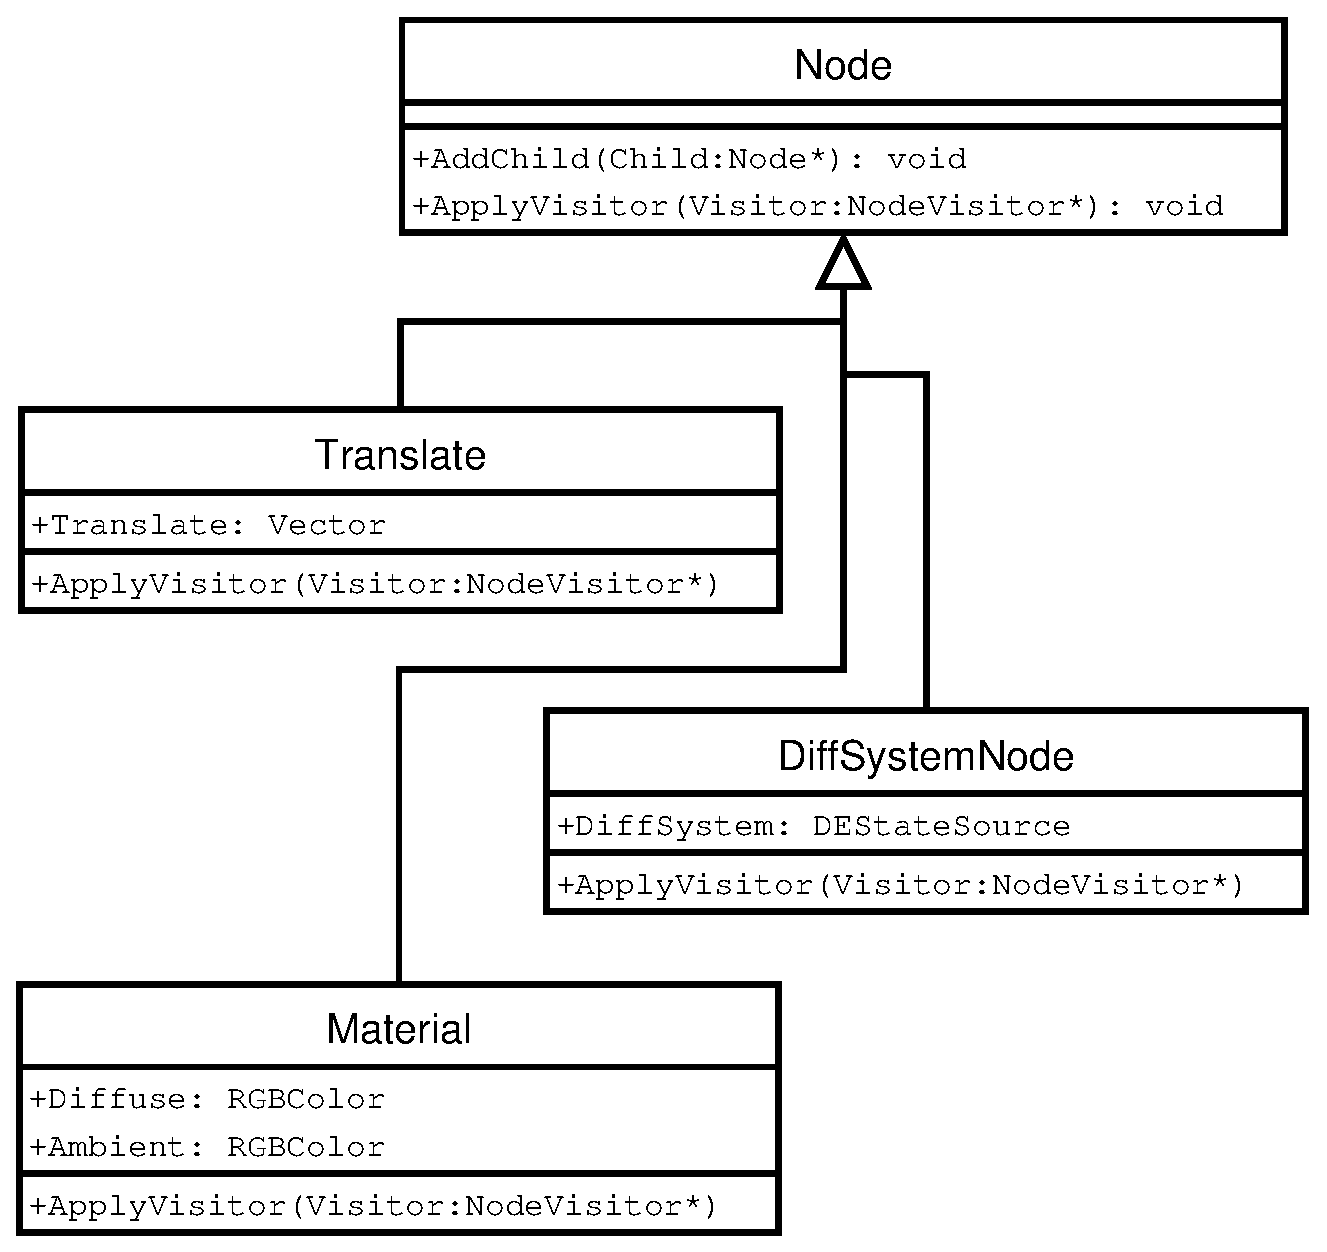
\includegraphics[height=0.5\textheight]{Node}    
    \caption{\label{Fig:Node}Node class and some children}
\end{figure}

\begin{figure}
    \centering
    \includegraphics[height=0.5\textheight]{NodeVisitor}
    \caption{\label{Fig:NodeVisitor}NodeVisitor class and some of its children. Not all the member functions are shown.}
\end{figure}

\begin{figure}
    \centering
    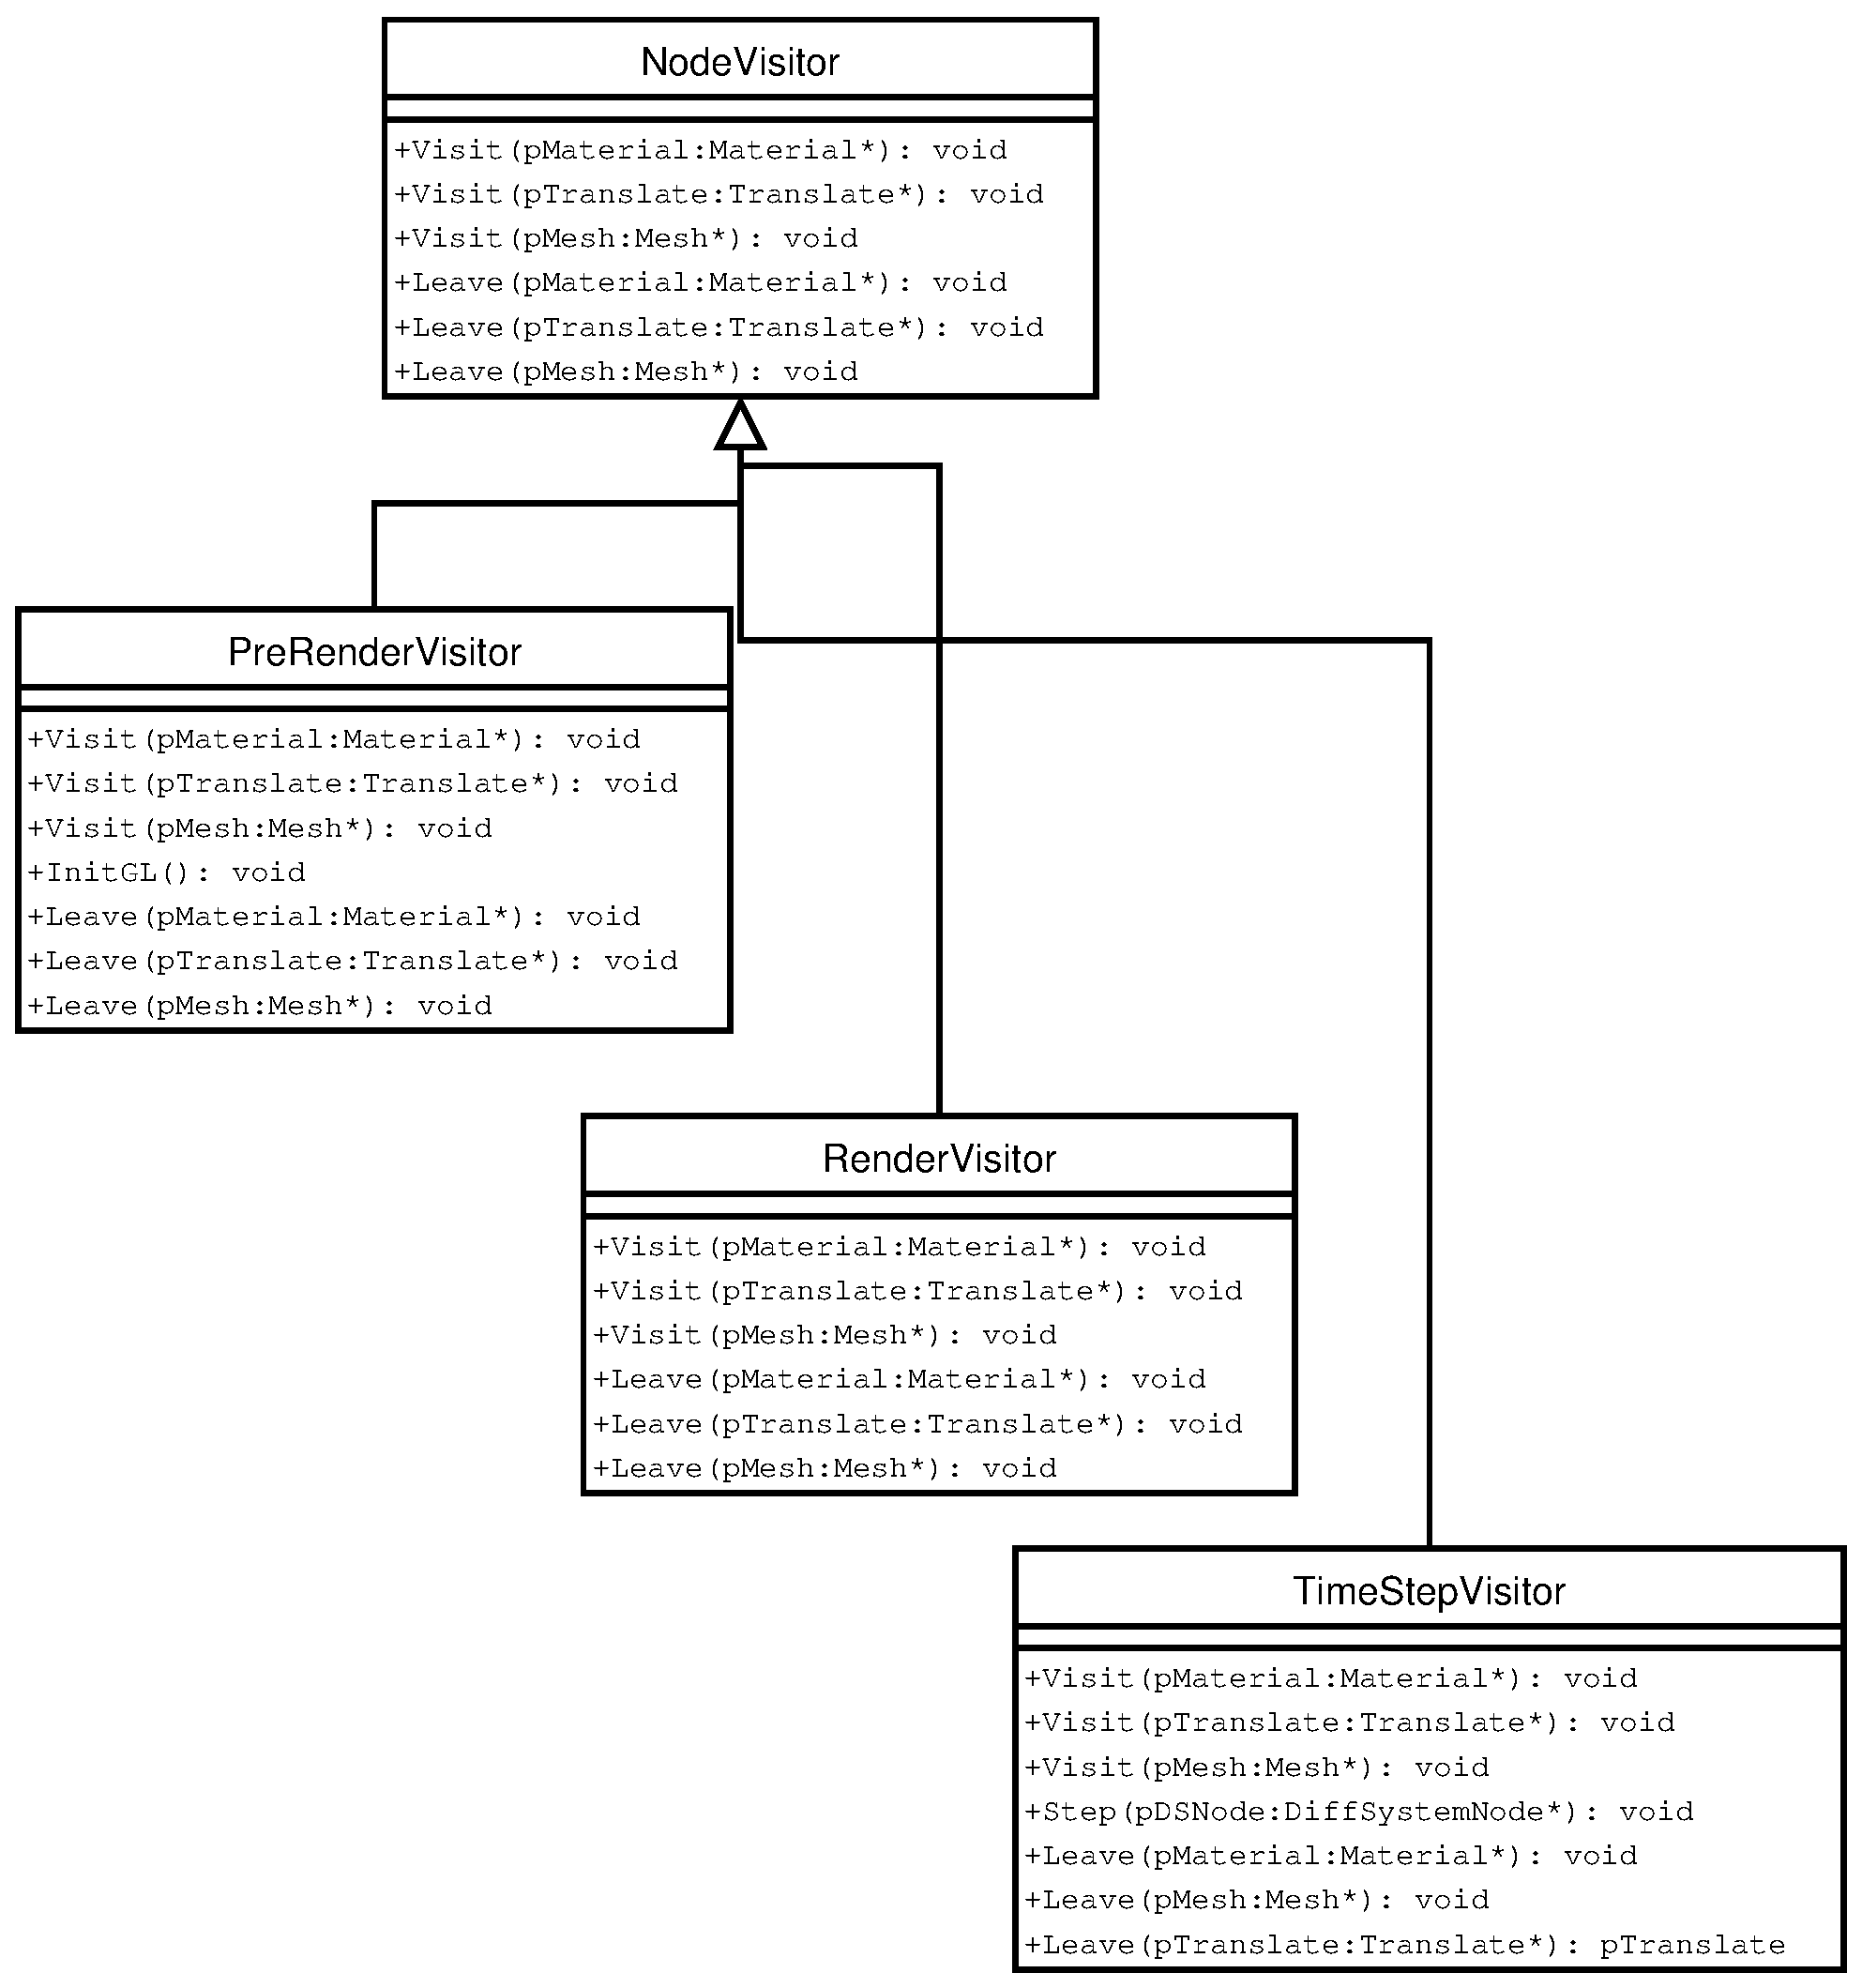
\includegraphics[height=0.8\textheight]{NodeVisitorOverloaded}
    \caption{\label{Fig:NodeVisitorOverloaded}NodeVisitor class with overloaded Visit and Leave member functions.}
\end{figure}

The net result is that the dynamic casting that occurs in listing \ref{Lst:DynCast}
can be replaced by the code show in listing \ref{Lst:OverloadCast}. This solution uses
overloaded functions to implement a form of compile time polymorphism.

\lstset{language=C++}
\begin{lstlisting}[basicstyle={\ttfamily \footnotesize},caption={Compile time polymorphism via member function overloading},label={Lst:OverloadCast}]
void TextureMap::ApplyVisitor(Edge::NodeVisitor* pVisitor)
{
  pVisitor->Visit(this);
  Node::ApplyVisitor(pVisitor);
  pVisitor->Leave(this);
}
\end{lstlisting}

The advantages of this approach is that the need for dynamic casting is
removed. Specifically we avoid accidently casting from a base
class to the wrong derived class. It also benefits efficiency since a virtual
function implies an extra level of indirection involved because the function to
call is looked up at runtime. An overloaded function does not
suffer this problem since the function to call is known at compile
time. Probably the most significant disadvantage of this strategy is that it
requires every class derived from \identifier{NodeVisitor} to implement the
\identifier{Visit} and \identifier{Leave} functions even if they are only stub
functions. Given that many classes can potentially exist that are derived from
\identifier{Node}, adding a new class, say \identifier{EnvTexNode}, that derives
from \identifier{Node} means implementing a corresponding \identifier{Visit} and
\identifier{Leave} member function for every class derived from
\identifier{NodeVisitor}. This is tedious work, however, since most of it is
boilerplate code, it may be possible to alleviate this by the clever application
of macros which automatically generate the stub functions in the cases where the
visiting object need not react with the \identifier{Node} derived class in
question.

\section{Pendulum}
This program demonstrates the system in action. A fixed position constraint and a
series of fixed distance constraints are arranged to simulate a pendulum. The
red ball is subject to a fixed position constraint. The other balls are subject
to a series of fixed distance constraints (see Figure \ref{Fig:Balls}).
\begin{figure}    
    \centering
	\includegraphics[width=1\textwidth]{Balls}    
    \caption{\label{Fig:Balls}Swinging Balls}
\end{figure}

\section{Verification}
Much effort was put into verifying the accuracy of the implementation. We did
this by comparing our results with those obtained via Mathematica and the
results printed in text books.

\subsection{Simple Pendulum}
Mathematica was used to verify some of the results generated by the programs written.
To verify that the algorithm was implemented correctly Mathematica was used to
solve the system of differential equations for a pendulum using Mathematica's
internal differential equation solving algorithms. A pendulum with a length of
1, mass of 1 and a force of -1 in the y direction was setup. The 
graphs of the x and y position of the particle are shown in figure
\ref{Fig:x_single_pendulum} and figure \ref{Fig:y_single_pendulum}.

\begin{figure} 
	\begin{center}
		\epsfig{file=./x_single_pendulum.pdf}
	\end{center}
    \caption{x value vs time (derived using Mathematica)}
\label{Fig:x_single_pendulum}   
%\end{figure}
%\begin{figure}    
	\begin{center}
		\epsfig{file=./x_single_pendulum_simple_constr.pdf}
	\end{center}
    \caption{x value vs time using simple constraint based dynamics}
	\label{Fig:x_single_pendulum_simple_constr}
\end{figure}  

Subsequently an implementation of a pendulum using the constraint formulation
given in \ref{Eqn:LambdaSimple} was implemented in C++. The numerical
integration technique used was RK4. The behaviour of the particle was expected
to be similar to the solution derived using Mathematica, and therefore the
graphs should look similar. It was not expected that the exact numerical values
be the same since Mathematica uses a more sophisticated algorithm to numerically
solve the differential equations than the RK4 solver implemented for this
thesis.  The graphs of the x and y positions are shown in figures
\ref{Fig:x_single_pendulum_simple_constr} and
\ref{Fig:y_single_pendulum_simple_constr}.

\begin{figure}    
	\begin{center}
		\epsfig{file=./y_single_pendulum.pdf}
	\end{center}
    \caption{Single pendulum. y value vs time (derived using Mathematica)}
	\label{Fig:y_single_pendulum}
%\end{figure}
%\begin{figure}    
	\begin{center}
		\epsfig{file=./y_single_pendulum_simple_constr.pdf}
	\end{center}
    \caption{Single pendulum. y value vs time using simple constraint based dynamics}
	\label{Fig:y_single_pendulum_simple_constr}
\end{figure} 

By looking at the graphs one can see that there is a great deal of similarity
between the motion of the pendulum derived using Mathematica and the motion
derived using constrained dynamics. For example compare figure
\ref{Fig:x_single_pendulum_simple_constr} and \ref{Fig:x_single_pendulum}. The
figure \ref{Fig:x_single_pendulum_simple_constr} shows the graph of the x position of the
pendulum that was generated using the constrained dynamics implementation. It is
very similar to figure \ref{Fig:x_single_pendulum} that shows the graph of the x
position derived using Mathematica. The graphs of the y position shown
in figures \ref{Fig:y_single_pendulum} and
\ref{Fig:x_single_pendulum_simple_constr} are also similar.

\subsection{Double Pendulum}
In order to verify that the generic constraints were working working in a
plausible manner a double pendulum system was implemented in three different
ways. The first way used Mathematica to solve the equations of motion using
Newtonian methods. The set of differential equations for $\Theta_1$ and
$\Theta_2$ (see \footnote{\url{http://www.myphysicslab.com/}}) was given to
Mathematica and a solution found using Mathematica's \identifier{NDSolve}
function.  Mathematica was employed again to solve the system using a Lagrangian
formulation of the double pendulum system.  Unexpectedly the solution was
slightly different depending on the technique used (i.e.  Newtonian or
Lagrangian). Evidence of this is shown in the graphs \ref{Fig:x1_newtonian},
\ref{Fig:x1_lagrangian}, \ref{Fig:y1_newtonian} and \ref{Fig:y1_lagrangian}. The
graphs show the movement of a double pendulum over time, initially set with both
angles at $\frac{\Pi}{8}$. Figure \ref{Fig:x1_newtonian} shows the x position of
the particle derived using Newtonian dynamics. The figure
\ref{Fig:x1_lagrangian} shows the x position of the particle when solved using
Lagrangian dynamics.  There are unexpected differences between the two graphs.
We were unsure what caused the difference, however speculate that it may be
because the double pendulum is a chaotic system. It may be possible that
numerical inaccuracy crept into the system when converting from angles to
positions in the case of the Newtonian simulation. The positions of the
particles are given by the following equations:
\begin{equation}
x_1 = L_1 \sin(\theta_1)
\end{equation}
\begin{equation}
y_1 = -L_1 \cos(\theta_1)
\end{equation}
\begin{equation}
x_2 = x_1 + L_2 \sin(\theta_2)
\end{equation}
\begin{equation}
y_2 = y_1 - L_2 \cos(\theta_2)
\end{equation}
In the Lagrangian case the positions come from the solution of the differential
equations because they are specified in terms of $\ddot{x_1}$, $\ddot{y_1}$,
$\ddot{x_2}$ and $\ddot{y_2}$. Errors can also creep in via the differential
equation solver. Two different sets of differential equations were solved using
\identifier{NDSolve} even though they represented the same double pendulum
system.
\begin{figure}
	\begin{center}
		\epsfig{file=./x1_newtonian.pdf}
	\end{center}
    \caption{\label{Fig:x1_newtonian}Double pendulum. x position of the 1st particle obtained using Newtonian methods}
	\begin{center}
		\epsfig{file=./x1_lagrangian.pdf}
	\end{center}
    \caption{\label{Fig:x1_lagrangian}Double pendulum. x position of the 1st particle obtained using Lagrangian methods}
\end{figure}

\begin{figure}
	\begin{center}
		\epsfig{file=./y1_newtonian.pdf}
	\end{center}
    \caption{\label{Fig:y1_newtonian}Double pendulum. y position of the 1st particle obtained using Newtonian methods}
	\begin{center}
		\epsfig{file=./y1_lagrangian.pdf}
	\end{center}
    \caption{\label{Fig:y1_lagrangian}Double pendulum. y position of the 1st particle obtained using Lagrangian methods}
\end{figure}

Finally the third method employed two fixed distance constraints and one fixed
position constraint. The matrix equation \ref{Eqn:LambdaStable} was solved using
a biconjugate gradient solver \cite{NumRecipes} and the resulting differential
system solved using a Runge-Kutta 4 implementation. The graphs of the motion of
the particle are shown in figures \ref{Fig:x1_constr_double_pendulum},
\ref{Fig:x1_double_pendulum}, \ref{Fig:y1_constr_double_pendulum} and
\ref{Fig:y1_double_pendulum}.  It was expected that the motion of the particles
be similar, but not exactly the same since the double pendulum is a chaotic
system. However, the graphs illustrate disconcerting differences between the
constrained dynamics implementation and the graph derived using Mathematica.
These differences are probably due to the the different differential equation
solver used. The constrained dynamics implementation used a Runge-Kutta 4
solver whereas Mathematica used \identifier{NDSolve}. Given that the double
pendulum is a chaotic system it would be susceptible to small numerical
differences.

\begin{figure}
	\begin{center}
		\epsfig{file=./x1_constr_double_pendulum.pdf}
	\end{center}
    \caption{\label{Fig:x1_constr_double_pendulum}Double pendulum. x position of the 1st particle
    obtained using a constrained dynamics implementation}
	\begin{center}
		\epsfig{file=./x1_double_pendulum.pdf}
	\end{center}
    \caption{\label{Fig:x1_double_pendulum}Double pendulum. x position of the 1st particle
    obtained using Newtonian methods and Mathematica}
\end{figure}

\begin{figure}
	\begin{center}
		\epsfig{file=./y1_constr_double_pendulum.pdf}
	\end{center}
    \caption{\label{Fig:y1_constr_double_pendulum}Double pendulum. y position of the 1st particle
    obtained using a constrained dynamics implementation}
	\begin{center}
		\epsfig{file=./y1_double_pendulum.pdf}
	\end{center}
    \caption{\label{Fig:y1_double_pendulum}Double pendulum. y position of the 1st particle
    obtained using Newtonian methods and Mathematica}
\end{figure}

\subsection{Testing the Differential Equation Solvers}
In order to verify that the differential equation solvers were working correctly
unit tests were setup using the Boost Test Library
\footnote{\url{http://www.boost.org/libs/test/doc/index.htm}}. The data for
testing the Euler solver was acquired from \cite[p. 120]{NagleSaff}. Data for
testing the Runge-Kutta solver was acquired from \cite[p. 135, p.
278]{NagleSaff}. The tables are shown below.
\newline
\newline
\begin{tabular}{|r|l|}
	\hline
	Step Size & Euler Approximation of $y = \dot{y}$\\
	\hline
	$1$ & $2.00000$ \\
	$10^{-1}$ & $2.59347$ \\
	$10^{-2}$ & $2.70481$ \\
	$10^{-3}$ & $2.71692$ \\
	$10^{-4}$ & $2.71815$ \\
	\hline
\end{tabular}
\newline
\newline
\begin{tabular}{|r|l|}
	\hline
	Time & 4th order Runge-Kutta approximation to $\ddot{y} + 3\dot{y} + 2y$\\
	\hline
	$0$ & $1.0000$ \\
	$0.125$ & $1.08989$ \\
	$0.250$ & $1.12334$ \\
	$0.375$ & $1.11713$ \\
	$0.500$ & $1.08383$ \\
	$0.625$ & $1.03277$ \\
	$0.750$ & $0.97984$ \\
	$0.875$ & $0.90304$ \\
	$1.000$ & $0.83297$ \\
	\hline
\end{tabular}

